\chapter{Employee turnover forecasting for human resource management based on time series analysis}\label{ch:timesereis}
\section{Introduction}
Prediction of employee turnover is a topic that has drawn the attention of researchers and human resource managers because employee turnover cost impacts both the operational capabilities and the budget of an organization. Employee turnover is both costly and disruptive to the functioning of most organizations, and both private firms and governments spend billions of dollars every year managing the issue according to \citet{leonard2001} . Furthermore, at crucial times, organizations find themselves short of niche skill-sets and resources which require time and planning to acquire. The lead time for hiring is often long, particularly when special skills are involved, and in some organizations like U.S. national laboratories, due to the security clearance requirements and training, the process could take months. Therefore, a good prediction of employee turnover at firm and departmental levels is essential for effective planning, budgeting, and recruiting in the human resource field. 

Human resource planning (HRP) is an ongoing process of systematic planning to achieve optimum use of the human resource pool in an organization. For an organization to execute their tasks efficiently and effectively, they need to ensure that the right people are available at the right places and at the right times to execute the tasks with the highest quality \citep{khoong1996}. Over the years, organizations have been able to scale up their efforts and success in manufacturing, marketing and financial plans. However, organizations have always struggled to develop sustainable HRP models \citep{heneman1993},. The objective of sustainable HRP models is to ensure the best match between employees and jobs to avoid manpower shortages or surpluses \citep{cambal2011}. To achieve this balance employee turnover is an important metric that is often central to organizations workforce planning and strategy.

As summarized in Table \ref{tab:1}, some of the previous studies attempt to identify the explanatory predictors of employee turnover. For instances, \citet{bluedorn1982} found that the turnover model appears to be related to the individual’s perception of environmental opportunities, routine, age, and the length of service. \citet{balfour1993} noticed that caseworkers with more education, less experience, and less stake in an organization are more likely to turnover. According to the research conducted by \citet{wright1998}, they found that emotional exhaustion was associated with both job performance and subsequent turnover, but not related to job satisfaction. \citet{morrow1999} used employee absenteeism and performance to predict employee turnover. The result from this study shows a positive correlation between absenteeism and voluntary turnover, and a negative correlation between performance ratings and voluntary turnover. The study conducted by \citet{thaden2010} indicated that organizational culture may potentially be an important factor to retain the workers in an organization. 
\begin{landscape}% Landscape page
\pagestyle{empty}%	
	\begin{table}[htbp]
		\centering
		\scriptsize
		\caption{Summary of Previous Research on Employment Turnover Forecast}
		\begin{tabular}{L{2.8cm}  L{2.8cm}  C{1.2cm}  L{3cm} C{1.2cm}  C{1.5cm} C{1.5cm} C{1.5cm}  L{2.8cm}}
			\toprule
			Authors (Year) & Data Acquisition &  Data Horizon & Methods & Software & Economic Indicator & Response Variable & Estimate & Model Evaluation \\
			\midrule
			Bluedorn (1982)& Employee records and Survey & 1 year & Correlations, multiple regression & N/A & No & Number & Point with intervals& $R^2=0.22$, Adjusted $R^2=0.11$ \\
			
			Ng et al. (1991) & Survey & N/A   & Hazard proportional model & BMDP 2L & No    &  Probability  & Point with intervals & Pair t-test  \\
			
			Balfour et al. (1993) & Employee records  & 33 months & Non-linear logistic regression & N/A   & No    & Probability  & Point & Chi-square values  \\
			
			Feeley et al. (1997) & Survey & 60 months & Social network, logistic regression, correlation & NEGOPY, UCINET & No    & Probability  & Point & $R^2=0.23$ \\
			
			Wright et al. (1998) & Survey & 1 year & Hypothesis test, correlation, logistic regression  & N/A   & No    & N/A   & N/A   & Correlation r=0.34, $P<0.01$ \\
			
			Morrow et al. (1999) & Demographic information and employee records & 2 years & Logistic regression, correlation & N/A   & No    & Probability  & Point & (-2 log likelihood) chi-square=193.13 \\
			
			Sexton et al. (2005) & Demographic information and employee records & 10 years (yearly) & NN    & FORTRAN  & Yes   & Leave or not & Point & Type I error=0.25\% Type II error=5.83\% \\
			
			Hong et al. (2007) & Survey & N/A   & Logit and probit model & SPSS  & No    & Probability  & N/A   & $R^2=0.5$, Quadratic Probability Scores = 0.18 for training and 0.12 for test \\
			
			Nagadevara et al. (2008) & Demographic information and employee records & 3 years & NN, logistic regression, classification/regression trees, discriminant analysis & N/A   & No    & Leave or not & Point & Contingency table \\
			
			Thaden et al. (2010) & Survey & 2 years & Multiple regression & N/A   & No    & Duration & Point with intervals &  $R^2=0.56$, $P< 0.001$ \\
			
			Größler and Zock (2010) & Employee records & 360 months & System dynamics  & N/A   & No    & Number & Point & N/A \\
			
			Saradhi et al. (2011) & Survey & 2 years & SVMs, random forest,  Naïve Bayes classifiers & N/A   & No    & Probability  & Point & True/false positive rate and precision \\
			
			Alao et al. (2013) &  Employee records   & 28 years (yearly) & Decision tree & WEKA See5 & No    & Probability  & Point & True/false positive rate and precision \\
			Tews et al. (2014) & Employee records and Survey & 6 months & Logistic regression & N/A   & No    & Probability & Point & $R^2=0.23$ \\
			Collini et al. (2015) & Survey and turnover rates   & 1 year & Correlation and Regression & N/A   & No    & Turnover rates & Point & No \\
			
			\bottomrule
		\end{tabular}%
		\label{tab:1}%
	\end{table}%
\end{landscape}
Other insights have been gained from some more recent research. For instance, according to \citet{tews2014}, personal events, professional events, internal work events and constituent attachment were highly related to turnover. \citet{collini2015} found that the interaction between interpersonal respect, mission fulfilment and engagement are statistically significant predictors for turnover in health care. However, diversity climate was not related with turnover. Finally, only \citet{sexton2005} considered outside economic variables, unemployment index and consumer price index, in the forecasting model for employee turnover; However, their final model did not include these two variables.
A recent editorial by \citep{ferrara2014} in the International Journal of Forecasting revealed new interest in forecasting business cycles with some complex methodologies. However, forecasting business cycle turning points is quite difficult, and \citet{hamilton2011} suggests that “the best econometricians can do is probably to nowcast recessions; that is, to recognize a turning point as soon as it occurs, or soon thereafter.”  Some type of outside variable might facilitate this situation.

Meanwhile, some other studies try to build turnover prediction models through techniques, such as regression, neural network (NN), and data mining. For example, \citet{ng1991} used a proportional hazards regression (PHR) to develop turnover prediction model and their forecasts are much more accurate. In the study conducted by \citet{sexton2005}, NN combining with modified genetic algorithm was used to build the prediction model for turnover. \citet{alao2013} applied decision tree skill on the employees’ demographical information and personnel records to identify attributes contributing to employee turnover.

In these studies, the data source was acquired either from human resource employment records and demographical information or survey with time horizon ranging from 1 to 28 years. Most of data is monthly data. It is worth mentioning that only few of these studies considered macro-economic factor in their prediction models, which could have significant impact on employee turnover.

Although there have been some efforts to predict employee turnover behaviour, no study has been conducted on turnover with time series forecasting skills, especially univariate time series forecasting, to predict employee turnover. In this study, the authors attempt to fill this gap. The advantage of time series forecasting approach is that it is not necessary to identify the determinants of turnover and helpful to evaluate the effects of either a planned or unplanned intervention \citep{velicer2003}.  
%Thus, this article has four parts. First, there is the introduction which covers the objective of the paper and a literature review. Second, there is a synopsis of tools for finding time series patterns and preparing the data for analysis as well as specific forecasting methods. The methods section is followed by the results and discussion of the study. Finally, there is conclusion of the results, practical implications, and limitations of the paper. 

\section{Methods}
\subsection{Data Preparation}
The human resource data was provided by a large multipurpose research organization in the U.S. The dataset consists of over 8,000 observations. These observations are active and terminated employees’ with incomplete demographic information from November 2000 to January 2012 including metrics such as payroll category, hired date, termination date, age, years of service, gender, job classification, and department code. The turnover dataset is summarized in the form of monthly data where each field represents the total number of employees leaving the organization. This dataset consists of 135 months spanning from November 2000 to January 2012. For this research, turnover is defined as total number of employees leaving the organization in each month. This definition of turnover is used as a unit of measurement for the turnover prediction. 

Several economic indicators have been examined in this study, such as, unemployment rate index, New York Stock Exchange, U.S gasoline price, and U.S monthly composite leading indicator (CLI). However, only CLI published by Organization for Economic Co-operation and Development (OECD) from November 2000 to January 2012 significantly improves the forecasting performance as a predictor of the cyclical component of employee turnover, since, in practice, CLI is used to give an early indication of turning points in the macro-economic cycle. CLI data used for this study was constructed by OECD through aggregating 7 components together. These 7 components include the number of dwellings started, net new orders for durable goods, share prices-NYSE composite, consumer sentiment indicator, the average weekly hours worked by manufacturing workers, the purchasing manager index, and spread of interest rates  \citep{oecd2013}. The authors have no information on weights of the index construction.
\subsubsection{Pattern Analysis, Cross-correlations, and Outlier Identification}
To model a time series, it is important to look for patterns in the turnover series.  First, this pattern analysis is simply addressed with a time plot of the series (a scatter plot over time) and box plots for the seasons or the months. In this case, the seasonal pattern of the turnover series is tested through Kruskal-Wallis and ANOVA tests ($P<0.05$), which do not correct for any trend in the series. The second stage of the pattern analysis is to use autocorrelation (ACF) and partial autocorrelation (PACF) plots to identify seasonal, autoregressive, and moving average patterns. If there are external variables (as in this case), the third stage of pattern analysis would be to examine the cross-correlations between ($Y_t$) and external variables (CLI ($X_t$) over time). The cross-correlation function (CCF) is used to identify lags of CLI ($X_t$) that might be useful predictors of turnover series ($Y_t$).  A longer lag that is strong enables the forecast horizon to be longer when using external variable. 

All of the previous stages of the pattern analysis could be contaminated by outliers so it is important to identify outliers before fitting the actual forecasting model. Box plot analysis by seasons can be used to informally flag outliers (this approach tends to over-identify outliers) while ARIMA methods in conjunction with statistical process control (SPC) tends to correctly identify the number of outliers in a series. Conservative ARIMA models ((1,0,1) or (0,1,1))  are used in this control charting. The residuals from ARIMA(1,0,1) are divided by the square root of mean square error to standardized them and the outliers are identified with the value greater than $\pm3$ standard deviations from zero by scatterplots of the standardized residuals \citep{alwan1988, grznar1997}.
Identifying the outliers using SPC and then smoothing them is a way to refine the data for further analysis and to facilitate finding the underlying pattern in the data series. Smoothing outliers in a time series is primary to filter out random noise and other irregularities. When the outlier is identified, it is adjusted to be more similar to its neighboring points \citep{grznar1997}. In this study, unusual observations were smoothed using a nonlinear data smoothing method, based on repeated medians (RMD) of a five period span (as shown in equation \ref{eq:1}) \citep{velleman1980}:
%equation1
\begin{equation} \label{eq:1}
	S_t=Median(y_{t-2s},y_{t-s},y_t,y_{t+s},y_{t+2s} ) 
\end{equation}
Where, $S_t$ is the actual smoothed value at time t, $y_t$ is value of response variable at time $t$, and $s$ is the number of total seasonal periods which is 12. This smoothing is only done on potential outliers within their season and not across adjacent periods. Sometimes outliers can distort normality, white noise, cross correlations, ACF and PACF, and the predictive performance of the model.  Thus, dealing with outliers properly means going back and asking hard questions about these unusual observations from a human resource perspective, and that can truly add understanding and improved forecasting ability.  It is always possible that the outliers are not always be unusual events but interventions or change points that need to be accommodated in the model.  In this kind of human resource dataset, such abnormalities could be retirement incentives were offered, another company was purchased, a section of the original company was sold off, or the potential outliers might reflect an economic down turn.  There are many possibilities; but if there is no over-identification of outliers, a good human resource department should be able to provide quick answers on the unusual situations.
\subsection{Time series analysis}
In time series forecasting, past observations of the same variable are collected and analysed to develop a model describing the underlying relationship. This modelling approach is particularly useful when little knowledge is available on the underlying data generating process or when there is no satisfactory explanatory model that relates the prediction variable to other explanatory variables \citep{zhang2003}. In this analysis, basically univariate time series methods are used to identify an optimum forecast with and without external variables. The statistical software used was Number Cruncher Statistical System (NCSS) and SAS. The turnover dataset is summarized by month and consists of 135 months spanning from November 2000 to January 2012 for conducting time series analysis. The data is analysed for two partitions of the data: training sample (November 2000 - January 2011) and holdout sample (February 2011 - January 2012). For each model, the training sample is used to build the model and the holdout sample is used for the validation of the model because the most recent time series data is considered the most important factor for prediction purposes \citep{bergmeir2012}. 
\subsection{Univariate Methods (without External Variables)}
These univariate time series analysis models use months and trend (for the most part) as predictors of turnover. The univariate models without external variables which were used in this study include time series regression, decomposition, Winter’s Exponential Smoothing (WES), and Box-Jenkins Autoregressive Integrated Moving Averages (ARIMA). One critical reason for using these kinds of time series models was so that there was not a constraint on the forecast horizon, i.e., how far in the future one could predict.

\subsubsection{Time Series Regression}
The univariate time series regression model adopts trend and seasonality as two predictors. The additive time series regression model with intercept, trend, monthly seasonality, and error terms takes the form as shown in equation \ref{equation:reg}:

\begin{equation}
	\label{equation:reg}
	Y_t = \beta_0+\beta_1 x_{trend} + \sum_{i=2}^{12} {\beta_i d_i}+\xi_i
\end{equation}

Where, $Y_t$ is the value of response variable at time $t$,  $\beta_i$ is the coefficients estimated by regression, $x_{trend}$ is a continuous variable representing trend with value from 1 to $n$, $d_i$ is dummy variable representing seasonal periods. In addition, the additive regression models with interventions: pulse or steps are also considered in the analysis due to the downsize policy in certain time points in our case, which are denoted by dummy variable in the regression function. The multiplicative time series regression model with intercept, trend, monthly seasonality, and error terms is also considered with the form as shown in equation \ref{eq:mulreg}
\begin{equation}
	\label{eq:mulreg}
	Ln(Y_t)=\beta_0+\beta_1 x_{trend} +\sum_{i=2}^{12} {\beta_i d_i}+\xi_i                              
\end{equation}

Where, $Ln(Y_t)$ is natural log transformation of $Y_t$. For these regression models, the significance of the model and the variables is examined by p-values at 0.05 significant level, lack of collinearity, and valid regression assumptions. 

\subsubsection{Decomposition}
Decomposition time series methods attempt to separate the series into four components: trend, cycle, seasonality, and irregularity. Decomposition methods can be described globally as equation \ref{eq:decom}. The decomposition model can be used assuming no cyclical variation or the cyclical variation can be extracted and a model fitted so that to enhance future forecasting. Of course, there can be quite complex decomposition models, but the classical multiplicative decomposition model in NCSS was used for my turnover series.
\begin{equation}
	\label{eq:decom}
	Y_t  =f(trend,cycle,seasonality,irregularity)=T_t  C_t S_t I_t            
\end{equation}

\subsubsection{Winters exponential smoothing (WES)}
WES models work well on series that either have seasonality or seasonality and trend.  The models can be additive or multiplicative as well, but the preferred option tends to have additive trend and either additive or multiplicative seasonality.  Multiplicative trend in these kinds of time series models tends to over or under forecast for future values. Of course, dampened models can help avoid this future forecast problem, but one must be careful then that the forecasts are short term \citep{de1998}. The robustness and accuracy of Winter’s exponential smoothing methods has led to their widespread use in applications where a large number of series necessitates an automated procedure \citep{win1960,tay2003}. WES model is easy to interpret and easily understood by management or those less technically inclined. 
\subsubsection{Autoregressive Integrated Moving Average (ARIMA)}
The ARIMA models were introduced by the statisticians George Box and Gwilym Jenkins \citep{box1970}. The general form of ARIMA models is ARIMA(p,d,q); where p, d, and q are non-negative integers that refer to the order of the autoregressive, integrated, and moving average parts of the model respectively. In addition, ARIMA models can handle seasonality, and their forms would be as follows: ARIMA(p,d,q)(P,D,Q). Thus, the seasonal aspect of a series could have an autoregressive, differencing, or moving average patterns as well.  ARIMA methods are popular to some forecasters because they provide a wide class of models for univariate time series forecasting \citep{har1983}.  

\subsection{Univariate methods (with external variables)}
Univariate models that incorporated an external variable (CLI) as a predictor of cyclical component of turnover series were also examined.  Basically, this included dynamic regression and more complex decomposition models.
\subsubsection{Dynamic regression with external variable}
The dynamic regression model describes how the forecasting output is linearly related to current and past values of one or more input series. There are two crucial assumptions for dynamic regression model. First, the observations of the input series are assumed to occur at equally spaced time intervals. Second, the input series are not affected by the output \citep{pankratz2012}. Dynamic regression models allow one to include external variables, interventions, and transfer functions. In this study, the external variables (CLI and interventions) are incorporated into the dynamic regression model. Equation \ref{eq:reg2} can be a simple representation of the model with trend, seasonal dummy variable, and interventions,
\begin{equation}
Y_t = \beta_0+\beta_1 x_{trend} + \sum_{i=2}^{12} {\beta_i d_i}+\varpi_0 I_t +\frac{\varpi_1}{1-\delta_1 B} I^{'}_t +\xi_i
\label{eq:reg2}
\end{equation}
where $I_t$ is dummy variable representing pulse and step periods, and $I^{'}_t$ is dummy variable representing pulse periods. Also, $\varpi_0$, $\varpi_1$, and $\theta_1$ are the change point coefficients estimated by regression and $1-\delta_1 B$ refers to the delayed rise or fall in the forecast variable.
  
\subsubsection{Decomposition with external variable}
In this more complex decomposition model, CLI and its lag terms are used as a predictor of cyclical component in the decomposition model. This research applies two approaches to obtain a decomposition model: one is the decomposition built in NCSS with the cyclical variable (CLI) incorporated and the other is a multiplicative decomposition model built by the product of the best ARIMA and cyclical factor (CLI). 
\subsection{Nonlinear and Multivariate Methods}
\subsubsection{State Space Model}
A state space model consists of an observation equation as shown in equation \ref{eq:ssm1} and a Markovian transition equation as shown in equation \ref{eq:ssm2} 
\begin{equation}
y_t=F_t \theta_t +v_t
\label{eq:ssm1}
\end{equation}
\begin{equation}
\theta_t=G_t\theta_{t-1} + w_t
\label{eq:ssm2}
\end{equation}
where $y_t$ is a $m \times 1$ data vector; $θ_t$  is a p×1 unknown state-vector, $F_t$ is a $m\times p$ state vector relating the observation data to the state vector $θ_t$, and $G_t$ is a $p\times p$ state transition matrix. In addition, $v_t$, $w_t$ are random error matrices which independently and identically follow a multinomial distribution. State space models are modelled using R “stats”, “dlm”, and “forecast” packages. 

\subsubsection{Vector Autoregressive Model}
Vector autoregressive model (VAR) is an econometric model for multivariate time series analysis. It is an extension of the univariate autoregressive model, i.e., each variable is represented as a linear function of its lags and lags of the other variables. VAR models are often used to describe and forecast financial and economic time series. A VAR model consists of a set of k variables (also called endogenous variables) $y_t=〖(y_{1t}, y_{2t}, \dots, y_{kt})$, denoted as $k\times1$ vector. A $p^th$ order VAR model is 
\begin{equation}
y_t=c+A_1y_{t-1}+\dots +A_py_{t-p}+e_t
\end{equation}
where there are $pA_i(k \times k)$ coefficient matrixces. Also, $e_t$  is a $k \times 1$ unobservable white noise vector process where expectation value of this vector is zero and time invariant covariance matrix $E(e_t e_t^{'})=\sum$. The VAR model is modelled by R “vars” package.
\subsection{Model Evaluation}
A good forecasting model should be evaluated on predictive ability, goodness of fit using the $R^2$ value, mean absolute percentage error (MAPE), mean absolute error (MAE) or other fit diagnostics, normality tests on residuals, and a white noise test on those same residuals to make sure that no pattern is left. The best fitting model is generally selected with higher $R^2$ value in the holdout data, lower MAPE, normally distributed residuals, and a passed white noise test.

(1) Pseudo$R^2$

For evaluation of the time series methods, the pseudo $R^2$ for training and holdout data is calculated as standard criteria to test the goodness of model fitting taking the form in equation \ref{eq:rsquare}.
\begin{equation}
	\label{eq:rsquare}
	R_{pseudo}^2=1-\frac{\sum_{t=1}^{n}(y_t-\hat{y_t})}{\sum_{t=1}^{n}(y_t-\bar{y_t})}
\end{equation}

(2) Mean absolute percentage error

MAPE is the other measure of accuracy of the time series model fitting methods as shown in equation \ref{eq:mape} \citep{Hanke1998, Bowerman2005}. This criterion is used to compare the model performance for the specific dataset by using time series methods, since it measures relative performance \citep{Chu1998}.
\begin{equation}
	\label{eq:mape}
	MAPE=\frac{\sum_{t=1}^{n}\left | \frac{y_t-\hat{y_t}}{y_t} \right |}{n}\%
\end{equation}

(3) Normality test

A good time series model should have normally distributed residuals. In this paper, normality of residuals is evaluated by two powerful normality tests: Shapiro-Wilk \citep{Shapiro1965} and D'Agostino Omnibus normality test \citep{d1990} in NCSS.

(4) White noise test

The white noise test is performed on the residuals to evaluate whether there might be some time series pattern remaining in the dataset not accounted for the model and result in independent residuals, random scatter, or no more time series pattern in residuals \citep{Weisent2010}. In practice, the Q-statistic (also called Box-Pierce statistic or Ljung-Box statistic) is used as an objective diagnostic measure of white noise for a time series to compare whether the autocorrelations from residuals and white noise are statistically significantly different. This test statistic is illustrated in equation \ref{eq:white}; where $k$ is selected to be about the lesser of two seasonal cycles, about one-fourth of the observations, or 24 when two seasonal cycles is much greater than 24. In most cases, if a model is lacking in white noise, it means this model is deficient and has to be rectified \citep{de1998}. 

\begin{equation}
	\label{eq:white}
	Q=n(n+2)\sum_{i=1}^k{\frac{ACF(i)^2}{n-i}}
\end{equation}
%%%%%%%%%%%%%%%%%%%%%%%%%%%%%%%%%%%%%%%%%%%%%%%
%%%%%%%%%%%%%%     Time Series Result and discussion   %%%%%%%%%%%%%%%%%
%%%%%%%%%%%%%%%%%%%%%%%%%%%%%%%%%%%%%%%%%%%%%%%
\section{Results and Discussion}
\subsection{Temporal Patterns of Employ Turnover and Outlier Identification}
The time based turnover series was restructured in a format so that it could be analysed to observe patterns like trend or seasonality and understand any inherent time series in the data for further investigation in that direction. As shown in Figure \ref{fig:1} (a), there is obvious seasonality pattern in the series. The box plot for turnover series from ANOVA test confirmed this seasonality pattern. In addition, there is a decreasing trend from January to November as shown in Figure \ref{fig:1}, and then the trend line rises up in December. The points with year label in Figure \ref{fig:1} (b) are considered as outliers, since they are beyond the upper whiskers. After all ARIMA models were tested, three outliers appeared in SPC chart (as shown in Figure \ref{fig:2}); and two of these three were also flagged by the box plot analysis. Combining the outliers identified by ANOVA test and SPC, 7 outliers are smoothed to soften their impact. The outliers include the turnover numbers for December 2001, March 2008, April 2008, May 2008, June 2008, August 2008, and September 2008. Whenever one has outliers, one needs to investigate the cause. For instance, December 2001 is a 9/11 lag impact on job hiring with stronger background checking and increased retiring/hiring. The outliers in 2008 reflect the downsizing policy issued in January 2008 with three months response time window to accommodate a voluntary reduction in workforce from the organization. 
\begin{figure}
	\centering
	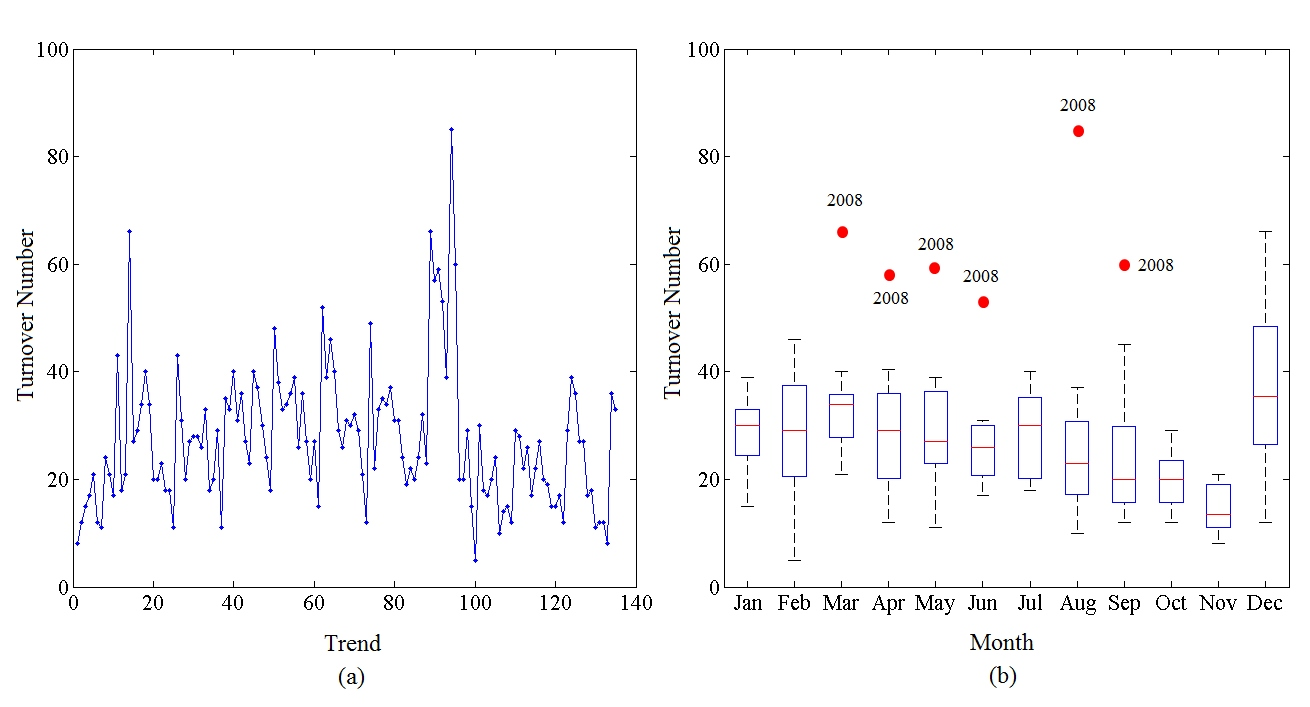
\includegraphics[width=5.5in]{Fig1.jpg}
	\caption{(a) Monthly Turnover Series Plotted Over Time and (b) Box Plot of Turnover Data.}
	\label{fig:1}
\end{figure}

\begin{figure}
	\centering
	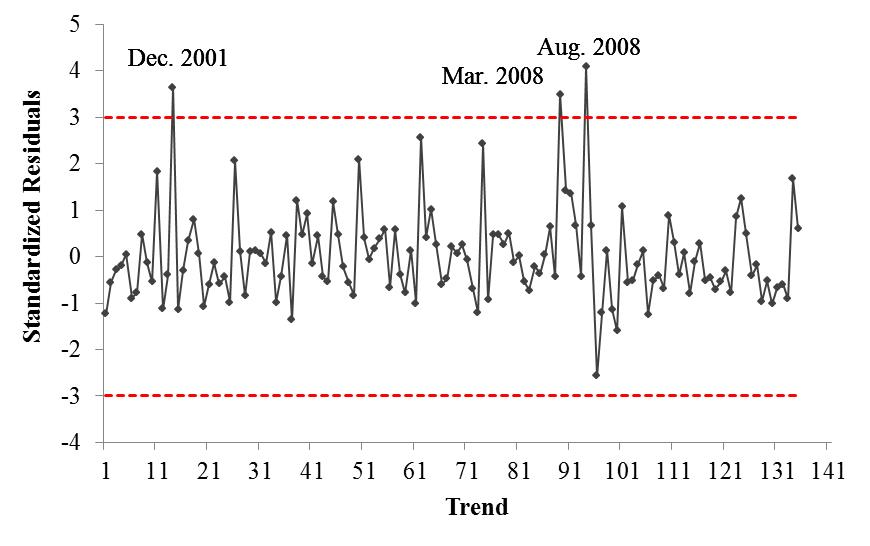
\includegraphics[width=5.5in]{Fig2.jpg}
	\caption{SPC Chart for Standardized Residuals.}
	\label{fig:2}
\end{figure}
The ACF and PACF plots for the turnover series are shown in Figure \ref{fig:3} (a, b). The pattern of unsmoothed data in the ACF and PACF hints at ARIMA(1,0,1) with some type of seasonality, but the seasonal pattern is not obvious.
\subsection{Cross-correlations}
The cross-correlation is employed between turnover series and CLI series to identify significant lag correlations. The cross-correlations between first differences for turnover and the CLI series were examined \citep{de1998}, and a “pre-whitening” process for the two series was used to identify the cross-correlation patterns \citep{box1970, bowie1981}.
% Department of Sciences at Pennsylvania State University, 2014).
Based all these calculation, CCFs from Lag 0 to Lag 8 are statistically significant, which indicates that the turnover series has statistically significant correlation with CLI and its 8 lags. The CLI and its 8 lags are applied into the dynamic regression, decomposition, and ARIMA model respectively as cyclical factor for forecasting.  

\begin{figure}
	\centering
	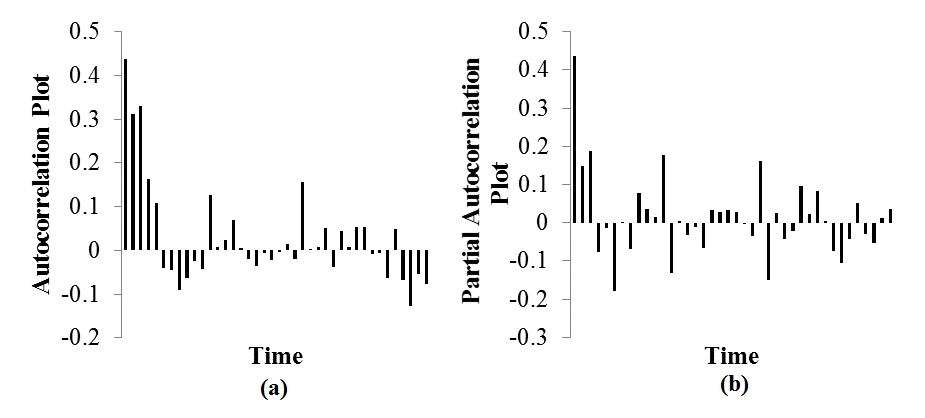
\includegraphics[width=5.5in]{Fig3.jpg}
	\caption{(a) Autocorrelation and (b) partial autocorrelation plots.}
	\label{fig:3}
\end{figure}


\subsection{Forecasting Results and Comparisons}
Forecasting evaluations for the time series models are provided in the Appendix Table \ref{tab:allmodels}, Table \ref{tab:dynamic}, Table \ref{tab:arima}, and Table \ref{tab:decomp}. Based on the evaluation statistics, 8 models are selected because of an acceptable $R^2$ value for the training and holdout data as well as their residual statistics that are the optimum among the other models (as shown in Table \ref{tab:1}).  On average, the holdout $R^2$ value of these models is 0.51 (range from 0.40 to 0.59). 
% Table generated by Excel2LaTeX from sheet 'Sheet1'
\begin{table}[htbp]
	\small %table fond
	\centering
	\caption{Statistics for Selected Time Series Models}
	\smallskip
	\begin{threeparttable}
		\begin{tabular}{C{2cm}p{0.5cm}m{5cm}C{0.8cm}C{1.5cm}ccc}%p: top m: middle
			\hline
			\multicolumn{1}{c}{Method} & \#    & \multicolumn{1}{c}{Model} & Pred $R^2$\tnote{1} & Holdout $R^2$& \multicolumn{1}{c}{MAPE}  & \multicolumn{1}{c}{Normality\tnote{2}} & \multicolumn{1}{c}{WN\tnote{3}} \\
			\hline
			\multirow{5}{2cm}{Univariate without external variable } & U1    & Regression with additive trend and seasonality & 0.51  & 0.57  & 26.15 & No    & No \\
			& U2    & Regression with additive trend, seasonality and intervention4  & 0.72  & 0.52  & 22.84 & Yes   & No \\
			& U3    & Decomposition & 0.65  & 0.54  & 17.97 & Yes   & Yes \\
			& U4    & WES with additive trend and seasonality & 0.52  & 0.52  & 20.65 & Yes   & Yes \\
			& U5    & ARIMA(1,0,1)(0,1,1) & 0.47  & 0.4   & 22.89 & Yes   & Yes \\  \hline
			\multirow{3}{2cm}{Univariate with external variable} & V1    & Dynamic regression using  lag7 CLI as predictor\tnote{4} & 0.77  & 0.59  & 19.91 & Yes   & Yes \\
			& V2    & Decomposition using  lag1 CLI as cycle & 0.65  & 0.55  & 17.97 & Yes   & Yes \\
			& V3    & ARIMA combining with lag1 CLI as cycle & 0.37  & 0.41  & 22.73 & Yes   & Yes \\
			\hline
		\end{tabular}%
		\begin{tablenotes}
			\item[1] Pred. $R^2$ is prediction $R^2$ value for training data.
			\item[2] Normality is residuals’ normality test.
			\item[3] WN is white noise test
			\item[4] The data is unsmoothed (or outliers are unadjusted) so as to take advantage of time series models that can accommodate interventions.
		\end{tablenotes}
	\end{threeparttable}
	\label{tab:1}%
\end{table}%

\subsubsection{Univariate Methods (	without External Variables)}
The regression model with additive trend and seasonality has the highest holdout$R^2$ (0.57) among the univariate models without external variables, indicating the model’s ability to explain 57\% of the total variation of the holdout sample. It is statistically significant ($P<0.05$) for the model and parameters. However, the residuals are not normally distributed and the model does not pass the white noise test. 

The regression model with additive trend, seasonality, and interventions (pulse and step) performs well with a training  $R^2$ of 0.72 and a holdout $R^2$ of 0.52, indicating the model’s ability to explain 72\% of the total variation of turnover for the training data and 52\% of the total variation of the holdout sample. It is statistically significant ($P<0.05$) for the model and parameters. The model has normally distributed residuals, but it does not have white noises. However, this regression model can capture the spike in December 2001 and sharp fluctuations from March 2008 to August 2008 (as shown in the Figure \ref{fig:4}). 
\begin{figure}
	\centering
	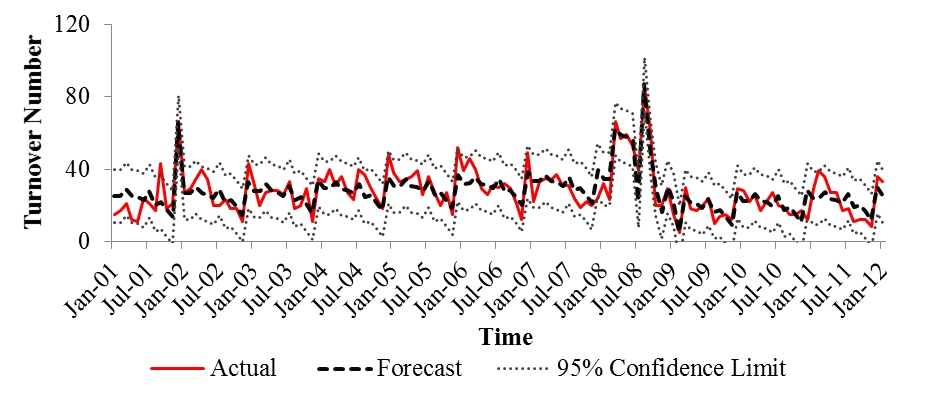
\includegraphics[width=5.5in]{Fig4.jpg}
	\caption{Regression with Interventions Forecast vs. Actual Turnover Number Plot.}
	\label{fig:4}
\end{figure}
The decomposition model is considered as the best univariate model without external variables because this model has a reasonably high training $R^2$ value (0.65), a good holdout $R^2$ value (0.54), and low MAPE (17.97). The residuals of this model are normally distributed and have a white noise pattern. Figure \ref{fig:5} shows the predicted turnover based on the decomposition model and the actual turnover number for holdout dataset. This plot validates the holdout performance of the decomposition model as it is able to mimic the changes in trend and seasonality of the turnover and prediction is close to the actual turnover numbers. However, it does seem to under-forecast for the 6 months June through November.
\begin{figure}
	\centering
	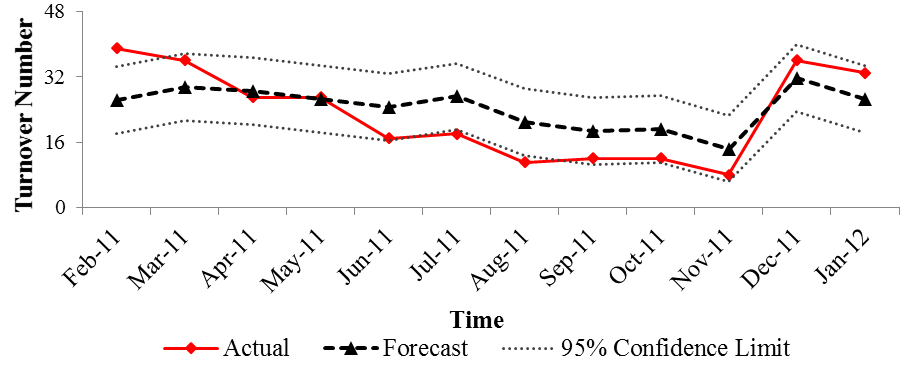
\includegraphics[width=5.5in]{Fig5.png}
	\caption{Decomposition Validation Forecast vs. Actual Turnover Number with Prediction.}
	\label{fig:5}
\end{figure}

\subsubsection{Univariate Methods (with External Variables)}
According to the cross-correlation analysis result, CLI and its 8 lags are applied in dynamic regression, decomposition model, and ARIMA(1,0,1)(0,1,1) respectively as external variable to forecast turnover number. The dynamic regression model with additive trend, seasonality, interventions (pulse and step), and lag7 of CLI is the best model among all models, since it has highest predicted and holdout  $R^2$ value (0.77 and 0.59), normalized residuals, and white noise. The dynamic regression is globally statistically significant and individually significant for the parameters ($P<0.05$).
\begin{figure}
	\centering
	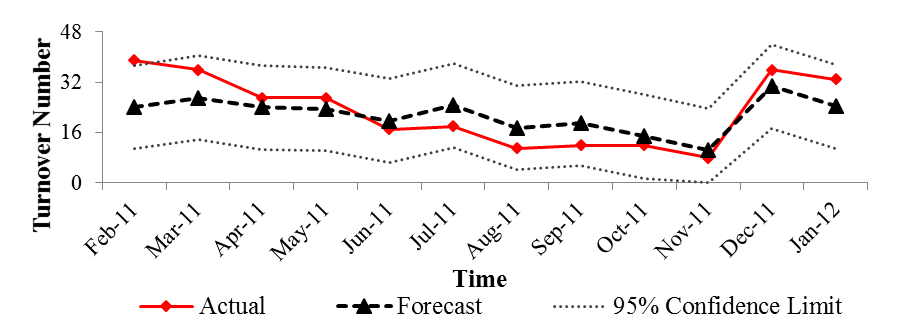
\includegraphics[width=5.5in]{Fig6.png}
	\caption{Dynamic Regression with Lag7 CLI Forecast vs. Actual Turnover Number for Holdout Dataset.}
	\label{fig:6}
\end{figure}
Figure \ref{fig:6} shows the predicted and actual turnover number plots for holdout dataset from dynamic regression model. Although there are under forecasts from July to September as well, the differences between forecasting value and actual value have become much tighter. Compared with top rated univariate methods without external variables, the performance of dynamic regression model is much improved after using CLI as an outside cyclical variable. 

\subsubsection{Nonlinear and Multivariate Methods (with External Variables)}
State space models with various combinations of errors, trend, seasonality, or an exogenous variable (CLI here) and VAR models of bivariate time series (turnover and CLI) are employed to forecast turnover number (as shown in Table 3). The exponential smoothing state space model with multiplicative error, no trend, and multiplicative seasonality has the highest holdout $R^2$ value (0.43) among all state space models, which is automatically selected by R forecast package from 27 exponential smoothing state space models. The residuals have white noise and are normally distributed. However, the training and holdout $R^2$ value (0.53 and 0.43) are relatively lower than the univariate regression models. 
Table 3 shows that the VAR models perform better than state space models. The VAR (4, constant, trend, and seasonality) is considered as the best among all these nonlinear and multivariate model with highest training and holdout $R^2$ value (0.62 and 0.64). The residuals are normally distributed and have white noise. However, variables in this model: lag terms of turnover and CLI are not statistically significant, indicating the model is over fitted. Only VAR (1, constant, trend, and seasonality) has significant lag 1 term of both turnover and CLI. This model also has higher training and holdout $R^2$ value (0.57 and 0.47) and white noise. However, its residuals are not normally distributed. 
The bivariate time series (turnover and CLI) does not have multivariate moving average pattern, which is not statistically significant. Therefore, the vector moving average (VMA) and vector autoregressive moving average (VARMA) methods are not employed to forecast. The volatility models (Garch (1,1) and stochastic volatility model) and nonlinear models (nonlinear autoregressive model and nonlinear threshold autoregressive model) have also been considered. However, all these models have lower training and holdout $R^2$ values and higher MAPE values. Their statistics are not provided in the Table \ref{tab:2} due to their poor performance.
\begin{table}[]
	\centering
	\caption{Statistics for Selected Nonlinear and Multivariate Models}
	\scriptsize
	\begin{threeparttable}
	\begin{tabular}{L{1.5cm}cL{3.5cm}ccccc}
		\toprule
		\multicolumn{1}{c}{Method} & \#    & \multicolumn{1}{c}{Model} & Pred. $R^2$ & Holdout $R^2$ & MAPE  & Normality & WN \\
		\midrule
		\multirow{6}[2]{*}{State Space} & S1    & Trend, Seasonality & 0.27  & 0.39  & 24.8  & No    & Yes \\
		& S2    & Trend, Slope, Seasonality & 0.23  & 0.32  & 28.58 & Yes   & Yes \\
		& S3    & Trend, Slope, Seasonality, CLI as regressor & 0.13  & 0.32  & 28.89 & Yes   & Yes \\
		& S4    & Exponential Smoothing (M,N,M) \tnote{1} & 0.51  & 0.43  & 21.14 & Yes   & Yes \\
		& S5    & Structural TS (Level, Slope)  & 0.46  & -0.16 & 22.82 & No    & No \\
		& S6    & Structural TS (Level, Slope, Seasonality)  & 0.51  & 0.04  & 21.47 & Yes   & Yes \\ \midrule
		\multirow{7}[2]{1.2cm}{Vector Autoregressive \tnote{2} } & VA1   & VAR(5, Constant, Seasonality) & 0.62  & 0.49  & 18.2  & No    & Yes \\
		& VA2   & VAR(5, Trend, Seasonality) & 0.63  & 0.52  & 18.37 & Yes   & Yes \\
		& VA3   & VAR(1, Constant, Trend, Seasonality) & 0.52  & 0.47  & 21.08 & No    & Yes \\
		& VA4   & VAR(2, Constant, Trend, Seasonality) & 0.59  & 0.44  & 19.63 & Yes   & Yes \\
		& VA5   & VAR(3, Constant, Trend, Seasonality) & 0.61  & 0.51  & 19.06 & Yes   & Yes \\
		& VA6   & VAR(4, Constant, Trend, Seasonality) & 0.62  & 0.64  & 18.44 & Yes   & Yes \\
		& VA7   & VAR(5, Constant, Trend, Seasonality) & 0.65  & 0.61  & 17.98 & Yes   & Yes \\
		\bottomrule
	\end{tabular}%
	\begin{tablenotes}
   \item[1]	M, N, M is multiplicative errors, no trend, multiplicative seasonality, respectively. 
   \item[2]	VAR(p) is pth order of  lag term. 
	\end{tablenotes}
	\end{threeparttable}
	\label{tab:2}%
\end{table}%
Even more non-linear and multivariate models were considered, but the intent of this research was not to go fishing for a best model but to find a simplistic model that could be used by human resource management (HRM).  It should be noted that a combination model might have been the better than our chosen dynamic regression model, but the authors were trying to keep it as simple as possible for HRM.
%%%%%%%%%%%%%%%%%%%%%%%%%%%%%%%%%%%%%%%
%%%%%    Time series analysis Conclusion  %%%%%%%%%%%%%%%%%%%
%%%%%%%%%%%%%%%%%%%%%%%%%%%%%%%%%%%%%%%
\section{Conclusion}
In this study, various univariate time series forecasting models for employee turnover prediction are tested and optimal models for In this paper, various time series forecasting models for employee turnover prediction are tested and optimal models for turnover forecasts are identified. The model in this paper actually performs better than those accessed in the literature review as a result of the external variable. Although VAR (4, constant, trend, and seasonality) has the highest holdout $R^2$, normally distributed residuals and white noise, dynamic regression model is concluded as the best forecasting model. There are several reasons why univariate methods are selected. In most cases, multivariate models help in generating more accurate model fit when compared to univariate models. However, univariate models are preferred as they are able to negate several drawbacks of multivariate models. For example, univariate models have less parameter uncertainty and less chance for outliers and errors due to their design simplicity. In most cases, univariate models are relatively easier to develop, interpret and get concrete conclusions. Multivariate models due to their complexity are more susceptible to misspecification. Besides, the explanatory variables in univariate models have to be determined accurately before forecasting the depending variable. Errors in forecasting the explanatory variable for a multivariate model may significantly affect the accuracy of the forecasts of the dependent variable when compared with an equivalent univariate model \citep{chatfield2000}. Apart from the benefits listed for univariate models, the dynamic regression model has several additional advantages. For example, an ARIMA error term which has autocorrelation pattern can be included in the model. Dynamic regression model is able to handle lagged regressors and various types of seasonalities. In addition, dynamic regression model can handle interventions or change points effectively, since these interventions or change points, such as holidays, promotions, new policy and so forth, are often common to the time series data. Thus, dynamic regression model could be used to forecast turnover for most of organizations of any size.  forecasts are identified. The model in the paper actually performs better than those accessed in the literature review. Dynamic regression model is concluded as the best forecasting model. Dynamic regression model has several advantages. For example, ARIMA error term which has autocorrelation pattern can be included in the model. Dynamic regression model is able to handle lagged regressors and various types of seasonality. In addition, dynamic regression model can handle interventions or change points effectively, since these interventions or change points, such as holidays, promotions, new policy and so forth, are often common to the time series data. Thus, dynamic regression model could be used to forecast turnover for most of organizations including small size, large size, and merged unit. However, to implement dynamic regression modelling, at least 5-years of monthly employee turnover data is preferred to make an accurate forecast. If the horizon of the dataset is less than 5 years, a special decomposition model \citep{ittig1997}could be considered as a substitute. Even though the forecasting horizon provided by dynamic regression model is relatively short, this is not a big issue for HR departments, since most of HR departments are only interested in a short term, such as three months, forecast. Therefore, if the HR department in an organization is not well familiar with forecasting techniques, dynamic regression model could be a good option for a preliminary turnover forecast once a CLI can be identified as in this paper. 

It is worth mentioning that an external variable like CLI in this paper does help in forecasting turnover since it does anticipate cyclical turning points. Incorporating such an external variable in the model is very helpful to get a good forecast when the HR department has a small and unreliable data set. Incorporating external variables, such as CLI, may help the whole forecasting process. If an external variable such as CLI is not available, a decomposition model could be considered as the first choice rather than dynamic regression model. In practice, some software such as NCSS or MINITAB have an embedded decomposition macro, which the HR departments could easily run given they knew how to estimate the cyclical variation.
\subsection{Practical implications}
\begin{itemize}
\item[(1)]	According to our findings, employee turnover forecast, in practice, could be handled easily. We suggest that HR departments could use regression model for the preliminary forecast and the accuracy of forecast is acceptable. However, there are some types of interventions that regression cannot handle, such as pulse or steps with exponential decay or growth. Dynamic regression is likely to be used as an alternative for forecasting.
\item[(2)] In this study, statistical analysis packages SAS and NCSS are used for the forecast. However, to some organizations, the HR departments are unwilling to spend extra funding on software purchase. Under this circumstance, Microsoft Excel could be a good alternative for the time series forecast without extra investment, because there have been some open source time series forecasting packages designed to run under Excel environment in the market. The forecasting models such as naïve model, moving average, exponential smoothing, decomposition, regression, and ARIMA model have been included into these packages \citep{warren2008}.
\item[(3)]	Another option these days is to use R for the dynamic regression \citep{hyndman2014}. The pseudo R code for dynamic regression and test on residuals (normality and white noise test) is provided below. 
\begin{lstlisting}
## Install R package
library (dynlm)
library (normwhn.test)
## Turnover is turnover data.  
## Trend is a continuous variable with value from 1 to n. 
## Seasonality is a dummy variable representing seasonal periods. 
## X is the lag term of CLI.
## Intervention is the external variable impact: yes=1 and no=0.
## Build model ## Load dataset
Turnover = read.xls (“turnover_data_in_excel.xls”)
## IMPORTANT: Some R codes in dynamic regression may not handle fancy intervention analysis.
Turnover.Model = dynlm (Turnover ~ Trend + Seasonality + L(CLI, X) + Intervention) 
## Model summary
summary ( Turnover.Model)
## Calculate residuals
Residual = resid (Turnover.Model)
## Normality test on residuals
normality.test1 (Residual)
## White noise test on residuals
whitenoise.test (Residual)
\end{lstlisting}
\end{itemize}
\subsection{Limitations and future research}
This study is limited to forecast total turnovers in an organization. It may be possible to apply univariate time series forecasting models to forecast turnovers in different categories like retirement or volunteer quit. Although the study incorporated CLI as an external factor and the accuracy of forecasts is well improved, the external factors affecting turnover can be much beyond the scope of CLI, as local and cyclical economic fluctuations strongly influence the propensity of employees to quit \citep{abelson1984}.

